% !TeX spellcheck = es_ES

\title[Prácticas ágiles]{Prácticas}
\date{}
\author[Pepe Doval]{}
\institute{}

\section{Prácticas}
\label{sec:Practicas}

\usebackgroundtemplate{%
  \tikz[overlay,remember picture] 
  \node[opacity=0.3 , at=(current page.south east),anchor=south east] {
    
\includegraphics[]{fondo}};
}

\begin{frame}
  \titlepage
  \begin{figure}[ht]
    \centering
    \vspace*{-2.5cm}
  \end{figure}
\end{frame}

\subsection{Prácticas habituales}
\label{subsec:Practicas}

\begin{frame}
  \frametitle{Al programar (1/2)}
  \begin{itemize}
    \item Pair programming
    \item TDD
    \item Refactorización
    \item Integración continua
  \end{itemize}
\end{frame}

\begin{frame}
  \frametitle{Al programar (2/2)}
  \begin{itemize}
    \item Diseño simple
    \item Propiedad colectiva del código
    \item Estándares y convenciones
  \end{itemize}
\end{frame}

\begin{frame}
  \frametitle{Al planificar (1/2)}
  \begin{itemize}
    \item Iteraciones
    \item Time boxing
    \item Planning game
    \item Standup meetings
  \end{itemize}
\end{frame}

\begin{frame}
  \frametitle{Al planificar (2/2)}
  \begin{itemize}
    \item Automatización
    \item Radiadores de información
    \item Definitions of done
  \end{itemize}
\end{frame}

\begin{frame}
  \frametitle{Al aprender (1/2)}
  \begin{itemize}
    \item Katas
    \item Coding Dojos
    \item Mob programming
    \item Desksurfing
  \end{itemize}
\end{frame}

\begin{frame}
  \frametitle{Al aprender (2/2)}
  \begin{itemize}
    \item Patrones de aprendizaje
    \item Mentoring
    \item Artesanía del software
  \end{itemize}
\end{frame}

\begin{frame}
  \frametitle{El ingrediente secreto}
  \begin{figure}[ht]
    \centering
    
\includegraphics[scale=0.15]{ingrediente_secreto}
    \caption{http://kungfupanda.wikia.com/}
  \end{figure}
\end{frame}

\begin{frame}
  \frametitle{Agile}
  \begin{figure}[ht]
    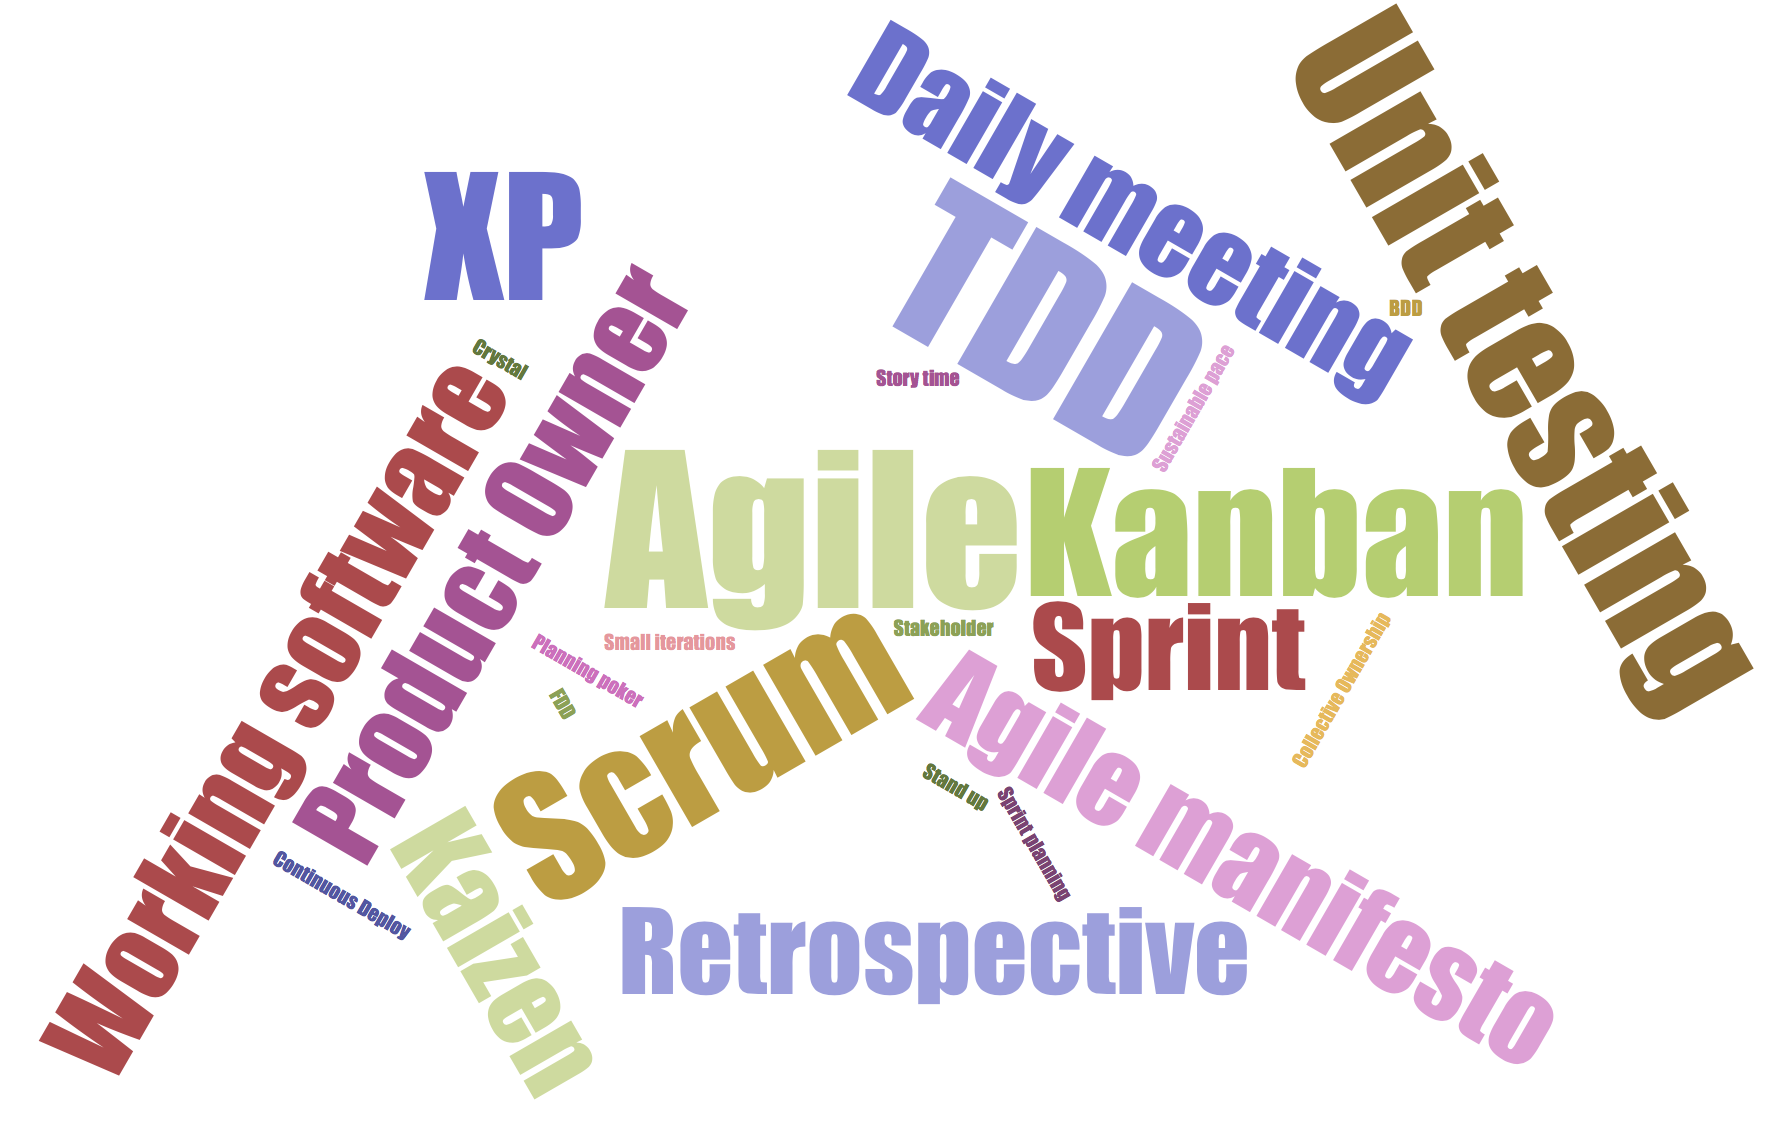
\includegraphics[scale=0.3]{cloud_agile}
  \end{figure}
\end{frame}
